\chapter{Science of ice reservoirs}
\label{chap:science}

\cleanchapterquote{I could do with some scientific help from specialists. I am trying to collect data on how and
	where glaciers form best so that I can improve on them and people can use the technique elsewhere.
}{Chewang Norphel}{(Padmashree awardee, Inventor of ice terraces)}

Given the importance of \ac{AIRs} in different mountainous regions, it is key to adequately understand their
functioning and to quantify their water storage at global scale. Addressing these research questions
calls for the use of holistic modelling frameworks in which all relevant processes are represented, including
components of the terrestrial hydrological cycle, human water management, atmospheric processes, and climate
change drivers, in a globally integrated way. In such coupled frameworks, interactions and feedback between
ice surface and climate are directly modelled and represented under different scenarios and for different time
periods, allowing the investigation of both the physical mechanisms and the spatial and temporal extents of water
storage. To date, glacial models have provided this type of integrated framework but without accurate
representations of \ac{AIRs}. However, with some modifications, glacial models can become ideal tools to estimate the
meltwater quantities of \ac{AIRs} for the historical and present-day periods and for scenarios of future
climate change. Such model-based assessments can aid future mitigation and adaptation strategies linked to AIR
construction and operation to assess future water scarcity and ensure future water availability in a changing
climate.

To achieve this, three physically based models of increasing complexity are developed in the present thesis to estimate
AIR volume evolution. The first one, referred to as Oerlemans model (Paper III), integrates a simple shape
evolution module to demonstrate that AIR volume estimations are possible using equations used for modelling
glacial surfaces. The second one, referred to as AIR model (Paper I), extends this approach to calibrate the
model parameters and validate the volume estimations it provided. The third one, referred to as COSISTUPA,
reduces model calibration overhead while providing a user-friendly framework to update model parametrizations
and apply the model to new construction sites. 

In this chapter, the datasets obtained across measurement campaigns in two different mountain regions (the Alps and
the Himalayas) are presented. Description of the shape evolution and mass and energy balance modules used to assess quantity of ice, meltwater, sublimation, and wastewater are also provided herein.
Finally, features and shortcomings of each model are compared.

\section{Study sites and data}

The study sites in the Alps and the Himalayas were chosen for two reasons. First, they enable a
comparative study between locations with considerable differences in meteorological characteristics. Second,
these locations do not present significant logistical hurdles, since both selected sites have dedicated
teams for construction and measurement campaigns.

The study period starts when the fountain is first switched on (start date) and ends when the respective AIR
either melts or brakes into several ice blocks (expiry date). Each AIR dataset was abbreviated based on the
construction strategy used, prefix of the country code, and suffix of the year of its expiry date
(Table \ref{tab:AIRs}). The construction strategies are distinguished based on whether they use fountain scheduling
strategies or not to regulate water supply. Fountain scheduling was set with a control valve that was automated
with optimal discharge rates computed using real-time meteorological input and location metadata. Those using fountain scheduling were
code named "automated", whereas the rest were code named "manual". All except one construction campaign used
manual construction strategies. Therefore, manual \ac{AIRs} are referred to without explicitly
specifying their construction strategy.

In total, 23 \ac{AIRs} were studied in these two regions across four winters. However, complete meteorological, water, and volume measurements were available for only four \ac{AIRs} located in
Guttannen, Switzerland and one in Gangles, India. Therefore,
only these AIR datasets are used in the following analysis. The rest AIR datasets are described in the
Appendix table \ref{tab:Ladakh_AIRs} and are used in later chapters for qualitative analysis.

\begin{figure}[htb]
	\centering
	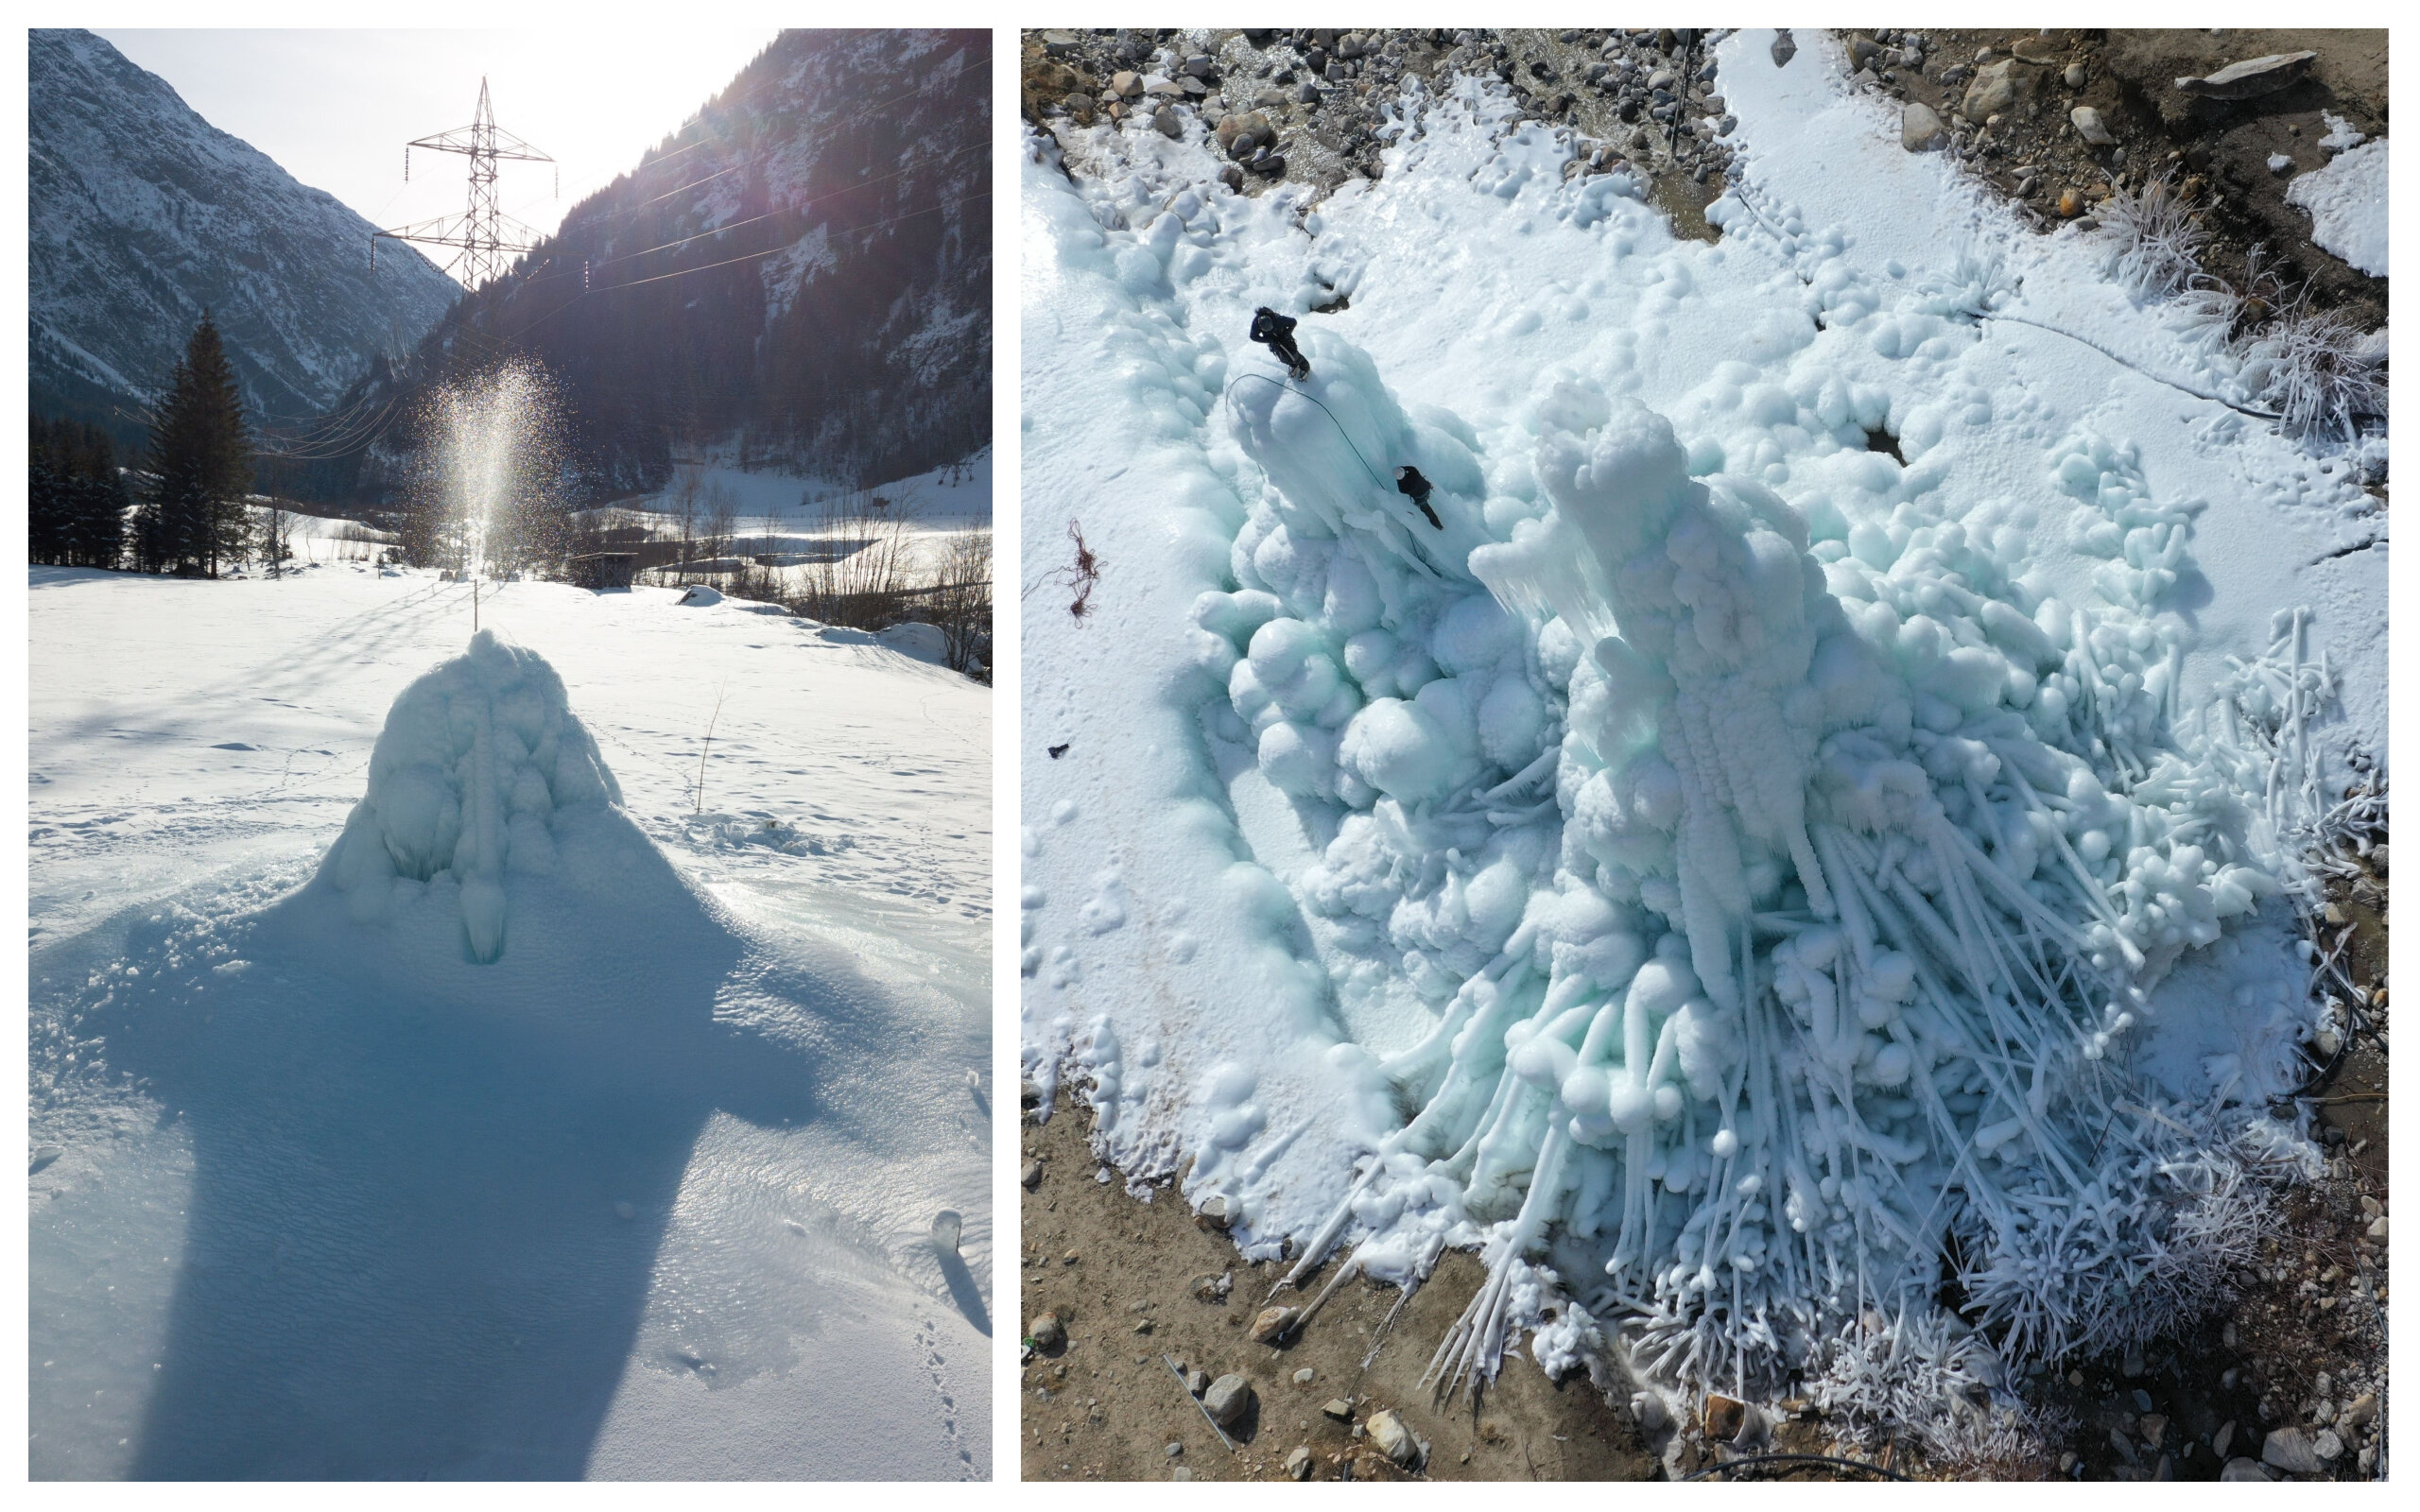
\includegraphics[width=12 cm]{figs/2AIRs.jpg}
	\caption{The Swiss and Indian \ac{AIRs} were 5 $m$ and 13 $m$ tall on January 9 and March 3, 2021,
    respectively. Photos: Daniel Bürki (left) and Thinles Norboo (right)}
	\label{fig:2AIRs}
\end{figure}

\subsection{Swiss site}

The Guttannen site (46.66 $\degree$N, 8.29 $\degree$E) is situated in the Berne region, Switzerland and presents an
altitude of 1047 $m$ a.s.l. In the winter (Oct–Apr), mean daily minimum and maximum air temperatures vary
between $-13$ and 15 $\degree C$. Clear skies are rare, averaging around 7 days during winter. Daily winter
precipitation can sometimes be as high as 100 $mm$. These values are based on 30 years of hourly historical
meteorological data series \citep{meteoblueClimateGuttannen2021}. Several \ac{AIRs} were constructed by the Guttannen
Bewegt Association, the University of Fribourg, and the Lucerne University of Applied Sciences and Arts during
the winters of 2020–22.

\subsection{Indian site}

The Gangles site (34.22 $\degree$N, 77.61 $\degree$E) is located around 20 km north of Leh city in the Ladakh
region, lying at 4025 $m$ a.s.l.. The mean annual temperature is $5.6 \, \degree C$, and the thermal range is
characterized by high seasonal variation. During January, the coldest month, the mean temperature drops to $-7.2
	\, \degree C$. During August, the warmest month, the mean temperature rises to $17.5 \, \degree C$
\citep{nusserIrrigationDevelopmentUpper2012}. Because of the rain shadow effect of the Himalayan range, the mean
annual precipitation in Leh totals less than 100 $mm$, and there is high interannual variability. While the
average summer rainfall between July and September reaches 37.5 $mm$, the average winter precipitation between
January and March amounts to 27.3 $ mm$ and falls almost entirely as snow. \ac{AIRs} were constructed here by the
Himalayan Institute of Alternatives, Ladakh during the winter of 2020/21.

\subsection{Meteorological data}

Air temperature, relative humidity, wind speed, pressure, longwave, and global shortwave radiation are required
as model input. The resulting dataset highlights the difference in meteorological influences driving ice
volume evolution in the two study sites ( Table \ref{tab:Observations}).

\begin{table}
	\centering
	\caption{Summary of the meteorological observations for \ac{AIRs} built during the respective study period.
		The meteorological measurements are shown using their mean ($\mu$) and standard deviation ($\sigma$) during the study
		period as $\mu \pm \sigma$. }

	\label{tab:Observations}
	\begin{tabular}{|lllll|}
		\hline
		\textbf{Name}        & \textbf{Symbol} & \textbf{IN21} & \textbf{CH21} & \textbf{Units} \\ \hline
		Air temperature      & $T_a    $       & $0 \pm 7$     & $2 \pm 6$     & $\degree C$    \\
		Relative humidity    & $RH     $       & $35 \pm 20$   & $79 \pm 18$   & \%             \\
		Wind speed           & $v_a        $   & $3 \pm 1$     & $2 \pm 2$     & $m/s$          \\
		Global shortwave     & $SW_{global} $  & $246 \pm 333$ & $138 \pm 243$  & $W\,m^{-2}$    \\
		Hourly precipitation & $ppt        $   & $0 \pm 0$     & $139 \pm 457$ & $mm$           \\
		Pressure             & $p_a         $  & $623 \pm 3$   & $794 \pm 9$   & $hPa$          \\\hline
	\end{tabular}
\end{table}

\subsection{Fountain observations}

A fountain consists of a pipeline and a nozzle. The pipeline has three attributes, namely discharge rate
($Q$), height ($h$), and water temperature ($T_F$). "Discharge rate" represents the discharge rate of the water in
the fountain pipeline. "Height" denotes the height of the fountain pipeline installed. "Fountain water temperature"
is the temperature of water droplets produced by the fountain.

The fountain nozzle has three characteristics, namely the aperture diameter ($dia$) and pressure loss
($P_{nozzle}$). "Pressure loss" denotes the loss of water head due to the fountain nozzle. Additionally,
the observed ice radius formed from the fountain water droplets is denoted as spray radius ($r_F$) (Fig.
\ref{fig:CH20_rad}).

\begin{figure}[htb]
	\centering
	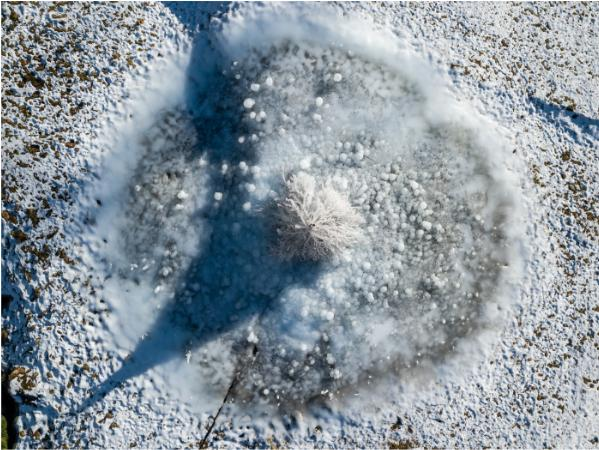
\includegraphics[width=\textwidth/2]{figs/CH20_sprayrad.jpg}
	\caption{Spray radius of the CH20 AIR }
	\label{fig:CH20_rad}
\end{figure}

\subsection{Drone flights}

\begin{table}
	\centering
	\caption{List of all \ac{AIRs} studied. The study period starts when the fountain is first switched on
		(denoted as Start Date) and ends when the respective AIR either melts or brakes into several ice blocks
		(denoted as Expiry Date). }
	\label{tab:AIRs}
	\begin{tabular}{|lllll|}
		\hline
		\textbf{Name}    & \textbf{Start Date} & \textbf{Expiry Date} & \textbf{No. of flights} & \textbf{Spray
		radius}                                                                                                 \\ \hline
		Manual CH20 & Jan 3 2020          & Apr 6 2020           & 2                       & 7.7 $m$       \\
		Manual CH21 & Nov 22 2020         & May 10 2021          & 8                       & 6.9 $m$       \\
		Manual IN21 & Jan 18 2021         & June 20 2021         & 6                       & 10.2 $m$      \\
		Manual CH22 & Dec 8 2021          & April 12 2022        & 8                       & 4.1 $m$       \\
		Automated CH22   & Dec 8 2021          & April 12 2022        & 6                       & 4.8 $m$       \\ \hline
	\end{tabular}
\end{table}


Several photogrammetric surveys were conducted for each \ac{AIR}. Details of these surveys and the
methodology used to produce the corresponding outputs are explained in paper I. The
\ac{DEMs} generated from the obtained imagery were analyzed to document the ice radius, the surface area, and the
volume of the ice structures. Ice radius measurements of drone flights which observed an increase in either AIR
circumference or volume were averaged to determine the fountain's spray radius. The number of drone surveys
conducted for each AIR and the corresponding spray radius observed are presented in Table \ref{tab:AIRs}.

\section{Model modules}
\label{sec:modules}

A bulk energy and mass balance model is used to calculate the amounts of ice, meltwater, water vapor, and
wastewater of the AIR. In each hourly time step, the model uses the AIR surface area, energy, and mass balance
calculations to estimate its ice volume, surface temperature, and wastewater, as shown in Fig. \ref{fig:schema}.

\begin{figure}
	\begin{center}
		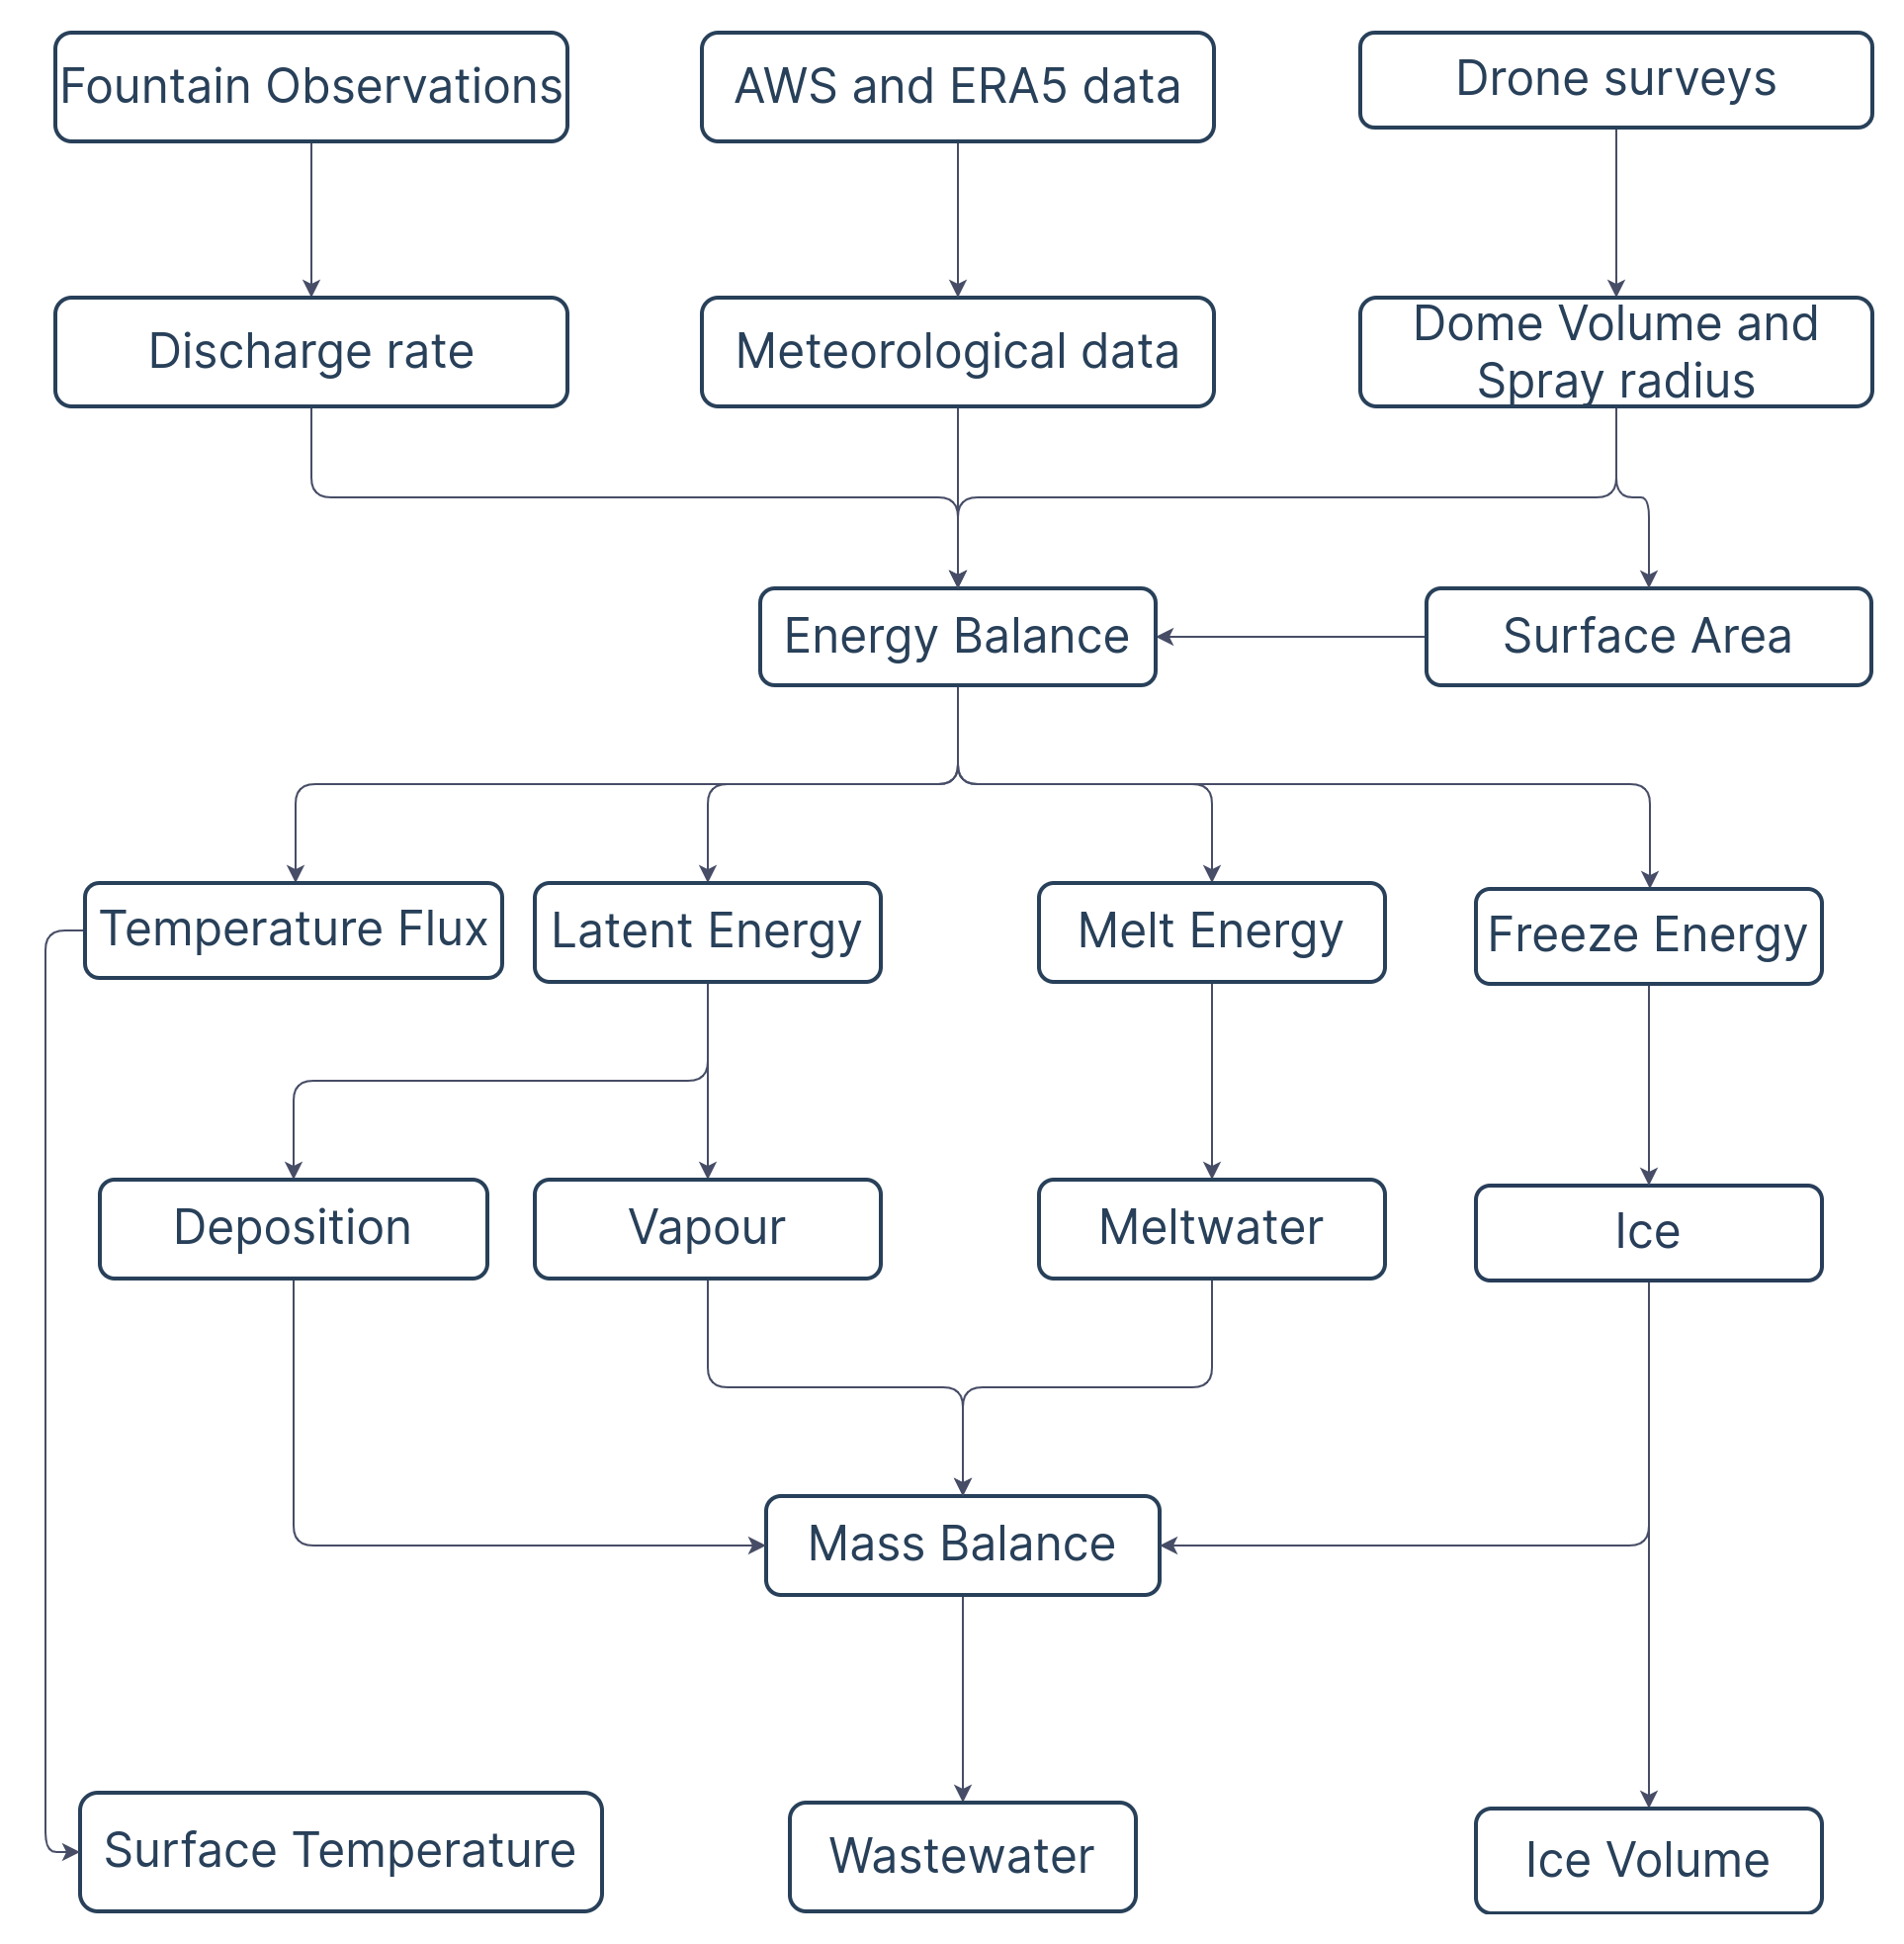
\includegraphics[width=10 cm]{figs/model_schematic.jpg}
	\end{center}
	\caption{Model schematic showing the workflow used in the model at every time step. }
	\label{fig:schema}
\end{figure}

\subsection{Shape evolution module} \label{sec:shape}

The model assumes the AIR shape to be a cone and assigns the following shape attributes:

\begin{subequations}
	\begin{align}
		\label{eq:A}
		A_{cone}^i & = \pi \cdot r_{cone}^i \cdot \sqrt{{(r_{cone}^i)}^2 + {(h_{cone}^i})^ 2} \\
		\label{eq:V}
		V_{cone}^i & = \pi/3 \cdot {(r_{cone}^i)}^2 \cdot h_{cone}^i                          \\
		\label{eq:thickness}
		j_{cone}^i & =\frac{\Delta M_{ice}^i}{\rho_{water}* A_{cone}^i}
	\end{align}
\end{subequations}

where $i$ denotes the model time step; $r_{cone}^i$ is the radius; $h_{cone}^i$ is the height; $A_{cone}^i$ is
the surface area; $V_{cone}^i$ is the volume, and $j_{cone}^i$ is the AIR surface normal thickness change as shown
in Fig. \ref{fig:shape}. $M_{ice}^i$ is the mass of the AIR, and $\Delta M_{ice}^i = M_{ice}^{i-1} -
	M_{ice}^{i-2}$. Henceforth, the equations used display the model time step superscript $i$ only if this is different
from the current time step.

AIR density can be defined as:

\begin{equation}
	\rho_{cone} = \frac{M_{F} + M_{dep} + M_{ppt}}{(M_{F} + M_{dep})/\rho_{ice} + M_{ppt}/\rho_{snow}}
\end{equation}

where $M_F$ is the cumulative mass of the fountain discharge; $M_{ppt}$ is the cumulative precipitation;
$M_{dep}$ is the cumulative accumulation through water vapor deposition; $\rho_{ice}$ is the ice density (917
$kg\,m^{-3}$) and $\rho_{snow}$ is the density of wet snow (300 $kg\,m^{-3}$) taken from
\cite{cuffeyPhysicsGlaciers2010}.

AIR volume can also be expressed as:

\begin{equation} V_{cone} =\frac{M_{ice}} {\rho_{cone}} \label{eq:V1} \end{equation}

The initial radius of the AIR is assumed to be $r_F$. The initial height $h_0$ depends on the dome volume
$V_{dome}$ used to construct the AIR as follows:

\begin{equation}
	h_{0} =  \Delta x + \frac{3 \cdot V_{dome}}{\pi \cdot (r_F)^2 }
	\label{eq:h0}
\end{equation}

where $\Delta x$ is the surface layer thickness (defined in Section \ref{sec:energy}).

During the subsequent time steps, the dimensions of the AIR evolve assuming a uniform thickness change ($j_{cone}$)
across its surface area with an invariant slope $s_{cone} = \frac{h_{cone}}{r_{cone}}$ .  During these time
steps, the volume is parameterized using Eqn. \ref{eq:V} as:

\begin{equation} 
  V_{cone} = \frac{\pi \cdot {(r_{cone})}^3 \cdot s_{cone}}{3} 
\label{eq:V2} 
\end{equation}

The ice stupa boundary is defined through its spray radius, i.e., ice formation is assumed negligible when
$r_{cone} > r_{F}$. Combining Eqns. \ref{eq:V},  \ref{eq:V1}, \ref{eq:h0}, and \ref{eq:V2}, the geometric
evolution of the ice stupa at each time step $i$ can be determined by considering the following rules:

\begin{equation} (r_{cone},\, h_{cone}) = \left\{ \begin{array}{ll} (r_F ,\, h_0)                                                                          & \textit{ if } i=0 \\
             (r_{cone}^{i-1},\, \frac{3 \cdot M_{ice}}{\pi \cdot \rho_{ice} \cdot {(r_{cone}^{i-1})}^2}) & \textit{ if }
             r_{cone}^{i-1} \geq r_{F} \textit{ and } \Delta M_{ice} > 0                                                     \\ (\frac{3 \cdot M_{ice}}{\pi \cdot \rho_{ice} \cdot s_{cone}})^{1/3} \cdot (1,\,  s_{cone}) &
             otherwise\end{array} \right.  \label{eq:A2} \end{equation}

\subsection{Energy balance module} \label{sec:energy}

\begin{figure}
	\begin{center}
		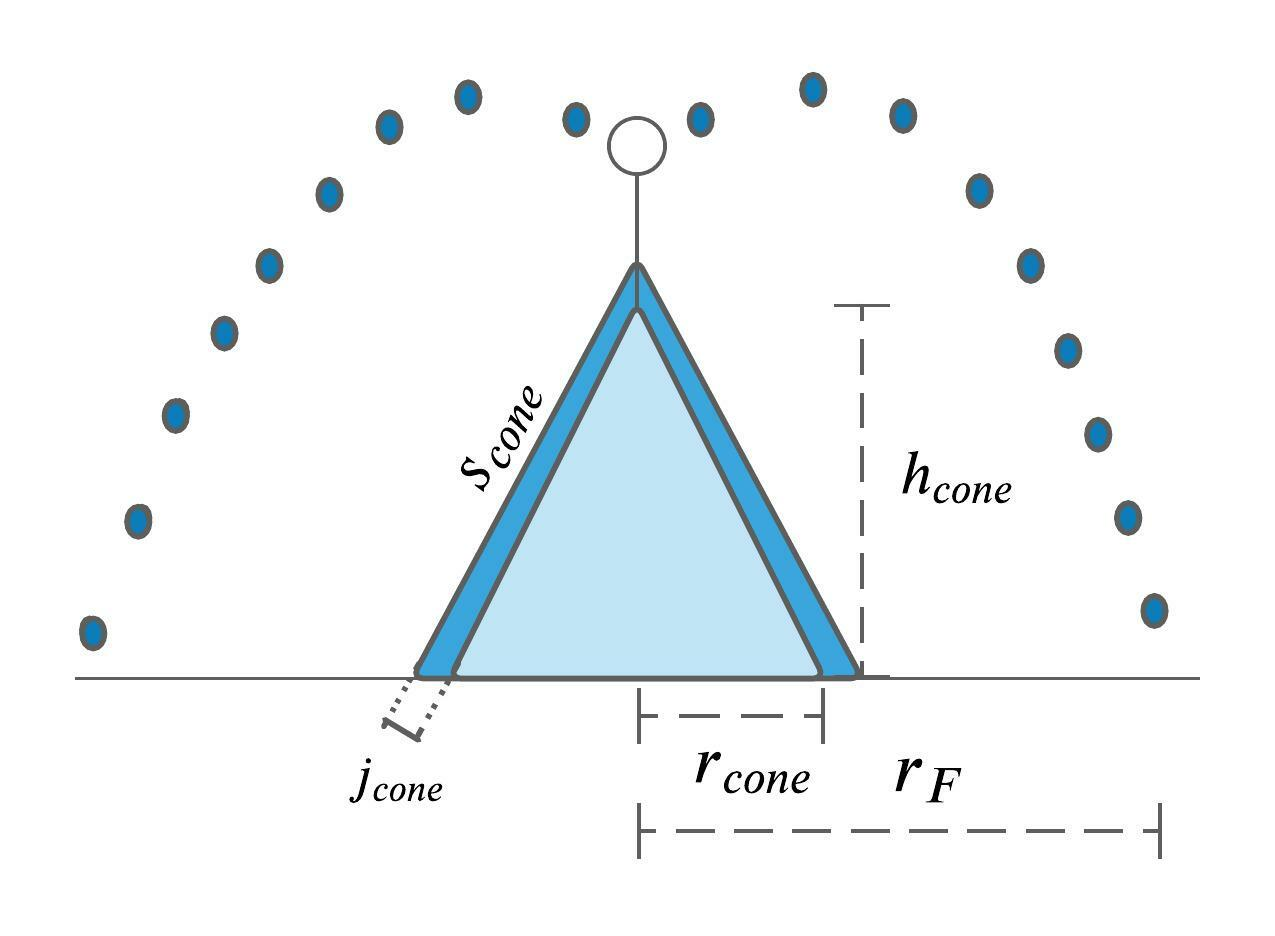
\includegraphics[width=10 cm]{figs/AIR_schematic.jpeg}
	\end{center}
	\caption{Shape variables of the AIR. $r_{cone}$ is the radius; $h_{cone}$ is the height; $j_{cone}$ is the
		thickness change, and $s_{cone}$ is the slope of the ice cone. $r_F$ is the spray radius of the fountain.}
	\label{fig:shape}
\end{figure}

The energy balance at the surface of an AIR is approximated by a one-dimensional description of energy fluxes
into and out of a (thin) layer with thickness $\Delta x$:

\begin{equation}
	\rho_{cone} \cdot c_{ice} \cdot \frac{\Delta T}{\Delta t} \cdot \Delta x = q_{SW} + q_{LW} + q_{L} + q_{S} + q_{F}+ q_{R} + q_{G}
	\label{eqn:EB}
\end{equation}

Upward and downward fluxes relative to the ice surface are positive and negative, respectively. The first term
is the energy change of the surface layer, which can be translated into a phase change energy should phase
changes occur. $q_{SW}$ is the net shortwave radiation; $q_{LW}$ is the net longwave radiation; $q_{L}$ and
$q_{S}$ are the turbulent latent and sensible heat fluxes, respectively. $q_{F}$ and $q_{R}$ represent the heat exchange of
the fountain water droplets and rain droplets with the AIR ice surface, respectively. $q_{G}$ represents bulk
heat flux between the AIR surface and its interior.

The energy flux acts upon the AIR surface layer, which has an upper and lower boundary defined by the atmosphere
and the ice body of the AIR, respectively. Here, the surface temperature $T_{ice}$ is defined to be the modelled
average temperature of the ice stupa surface layer.

\subsubsection{Net shortwave radiation \texorpdfstring{$q_{SW}$}{Lg}}

The net shortwave radiation $q_{SW}$ is computed as follows:

\begin{equation} q_{SW} = (1- \alpha)\cdot (SW_{direct} \cdot f_{cone} + SW_{diffuse}) \label{eqn:SW} \end{equation}

where $SW_{direct}$ and $SW_{diffuse}$ are the direct and diffuse shortwave radiation, respectively; $\alpha$ is the
modelled albedo, and $f_{cone}$ is the area fraction of the ice structure exposed to direct shortwave
radiation.

The albedo varies depending on the water source that formed the current AIR surface layer. During the fountain
runtime, the albedo assumes a constant value corresponding to ice albedo. However, after the fountain is
switched off, the albedo can reset to snow albedo during snowfall events and then decay back to ice albedo. We
use the scheme described in \cite{oerlemansYearRecordGlobal1998} to model this process. The scheme records the
decay of albedo with time after fresh snow is deposited on the surface. $\delta t$ records the number of time
steps after the last snowfall event. After snowfall, albedo changes over a time step, $\delta t$ , as

\begin{equation} \alpha=\alpha_{ice}+(\alpha_{snow}-\alpha_{ice}) \cdot e^{(-\delta t)/\tau} \label{eqn:alb}
\end{equation}

where $\alpha_{ice}$ is the bare ice albedo value (0.25); $\alpha_{snow}$ is the fresh snow albedo value (0.85),
and $\tau$ is a decay rate (16 $days$), which determines how fast the albedo of the ageing snow recedes back to
ice albedo. Discharge events decrease the decay rate by a factor of $\alpha_{ice}/\alpha_{snow}$.

The solar area fraction $f_{cone}$ of the ice structure exposed to direct shortwave radiation depends on the shape
considered. Using the solar elevation angle $\theta_{sun}$, the solar beam can be considered to present a vertical
component, impinging on the horizontal surface (semicircular base of the AIR), and a horizontal component,
impinging on the vertical cross section (a triangle). The solar elevation angle $\theta_{sun}$ used is modelled
using the parametrization proposed by \cite{woolfComputationSolarElevation1968}. Accordingly, $f_{cone}$ is determined as follows:

\begin{equation}
	\begin{split}
		f_{cone}& =\frac{(0.5 \cdot r_{cone} \cdot h_{cone}) \cdot cos \theta_{sun} +(\pi \cdot
		{(r_{cone})}^2/2) \cdot sin \theta_{sun} }{\pi \cdot r_{cone} \cdot ({(r_{cone})}^2+{(h_{cone})}^2)^{1/2}}\\
	\end{split}
	\label{eqn:f_{cone} }
\end{equation}

The diffuse shortwave radiation is assumed to impact the conical AIR surface uniformly.

\subsubsection{Net longwave radiation \texorpdfstring{$q_{LW}$}{Lg}} \label{sec:LW}

The net longwave radiation $q_{LW}$ is determined as follows:

\begin{equation}
	q_{LW}= LW_{in}-\sigma \cdot \epsilon_{ice} \cdot {(T_{ice}+ 273.15)}^4
	\label{eqn:LW}
\end{equation}

where $T_{ice}$ is the modelled surface temperature given in [$\degree C$];
$\sigma=5.67\cdot10^{-8}\,Jm^{-2}s^{-1}K^{-4}$ is the Stefan–Boltzmann constant; $LW_{in}$ denotes the incoming
longwave radiation, and $\epsilon_{ice}$ is the corresponding emissivity value for the ice stupa surface (0.97).

The incoming longwave radiation $LW_{in}$ for the Indian site, where no direct measurements were available, is
determined as follows:

\begin{equation}
	LW_{in}=\sigma \cdot \epsilon_a \cdot {(T_a+ 273.15)}^4
	\label{eqn:LWin}
\end{equation}

where $T_a$ represents the measured air temperature and $\epsilon_a$ denotes the atmospheric emissivity. The atmospheric emissivity $\epsilon_a$ is approximated using the equation suggested by \cite{brutsaertEvaporationAtmosphereTheory1982},
considering air temperature and vapor pressure (Eqn.  \ref{eqn:atm_e}). The vapor pressure of air over water and
ice is obtained using Eqn. \ref{eqn:vp}.  The expression defined in \cite{brutsaertDerivableFormulaLongwave1975} for clear skies
(first term in equation \ref{eqn:atm_e}) is extended with the correction for cloudy skies after
\cite{brutsaertEvaporationAtmosphereTheory1982} as follows:

\begin{equation}
	\epsilon_a=1.24 \cdot (\frac{p_{v,w}}{(T_a+273.15)})^{1/7}\cdot(1+0.22\cdot{cld}^2) \label{eqn:atm_e}
\end{equation}

with a cloudiness index $cld$, ranging from 0 for clear skies to 1 for complete overcast skies. For the Indian
site, cloudiness is assumed to be negligible.

\subsubsection{Turbulent fluxes} \label{sec:Qs}

The turbulent sensible $q_{S}$ and latent heat $q_{L}$ fluxes are computed with the following expressions
proposed by \cite{garrattAtmosphericBoundaryLayer1992}:

\begin{equation}
	q_{S}=\mu_{cone}\cdot c_{a} \cdot \rho_{a} \cdot p_{a}/p_{0,a} \cdot \frac{\kappa^2 \cdot v_a \cdot
		(T_a-T_{ice})}{{(\ln{\frac{h_{AWS}}{z_{0}}})}^2}
	\label{eqn:qs}
\end{equation}

\begin{equation}
	q_{L}=\mu_{cone}\cdot 0.623 \cdot L_s \cdot \rho_{a}/p_{0,a} \cdot \frac{\kappa^2 \cdot
	v_a(p_{v,w}-p_{v,ice})}{{(\ln{\frac{h_{AWS}}{z_{0}}})}^2}
\end{equation}

where $h_{AWS}$ is the measurement height above the ground surface of the \ac{AWS} (around $2\,m$ for all sites);
$v_a$ is the wind speed in [$m\,s^{-1}$]; $c_a$ is the specific heat of air at constant pressure (1010 J
$kg^{-1} K^{-1}$); $\rho_{a}$ is the air density at standard sea level (1.29 $kg m^{-3}$); $p_{0,a}$ is the air
pressure at standard sea level (1013 $hPa$); $p_{a}$ is the measured air pressure; $\kappa$ is the von Karman
constant (0.4); $z_{0}$ is the surface roughness (3 $mm$), and $L_s$ is the heat of sublimation (2848
$kJ\,kg^{-1}$). The vapor pressure of air with respect to water ($p_{v,w}$) and with respect to ice
($p_{v,ice}$) was obtained using the formulation given in \cite{huangSimpleAccurateFormula2018}:

\begin{equation}
	\begin{split}
		p_{v,w}&=e^{\frac{(34.494 - \frac{4924.99}{T_{a} + 237.1})}{(T_a + 105)^{1.57} \cdot 100}} \cdot \frac{RH}{100} \\
		p_{v,ice}&=e^{\frac{(43.494 - \frac{6545.89}{T_{ice} + 278})}{(T_{ice} + 868)^{2} \cdot 100}} \\
	\end{split} \label{eqn:vp}
\end{equation}

The dimensionless parameter $\mu_{cone}$ is an exposure parameter that deals with the fact that an AIR presents a rough
appearance and forms an obstacle to the wind regime. This factor accounts for the larger turbulent fluxes due to
the roughness of the surface \citep{oerlemansBriefCommunicationGrowth2021} and is a function of AIR slope
as follows:

\begin{equation}
	\mu_{cone} = 1 + \frac{s_{cone}}{2}
	\label{eqn:mu}
\end{equation}

The use of wind measurements from the horizontal plane at the \ac{AWS} can represent a possible source of error,
as these measurements might be different from those on a slope. However, this assumption is retained due to the absence of detailed datasets from the AIR surface.

\subsubsection{Fountain discharge heat flux \texorpdfstring{$q_{F}$}{Lg} } \label{sec:heatflux}

Fountain water temperature, $T_F$, is assumed to cool to 0 $\degree C$ after contact with the ice surface.
$T_F$ is equal to the measured source water temperature, but during time periods when the ambient temperature is
subzero, $T_F$ is assumed to be 0 $\degree C$. Thus, the heat flux caused by this process is:

\begin{equation}
	q_{F} = \left\{ \begin{array}{ll}
		\frac{ \Delta M_F \cdot c_{water} \cdot T_F}{\Delta t \cdot A_{cone}} & \textit{ if } T_{temp} > 0 \\
		0                                                                     & \textit{ otherwise}
	\end{array} \right.
\end{equation}

with $c_{water}$ as the specific heat of water (4186 J $kg^{-1} K^{-1}$).

\subsubsection{Rain heat flux \texorpdfstring{$q_{R}$}{Lg} }

The influence of rain events on the albedo and on the ice stupa's energy balance is assumed to be similar to that of discharge
events. However, the water temperature of a rain event is assumed to be equal to the air temperature. Accordingly,
the heat flux generated due to a rain event is determined:

\begin{equation}
	q_{R} = \frac{ \Delta M_{ppt} \cdot c_{water} \cdot T_a}{\Delta t \cdot A_{cone}}
	\label{eqn:qR}
\end{equation}

\subsubsection{Bulk heat flux \texorpdfstring{$q_{G}$}{Lg}} \label{sec:Bulkflux}

The bulk heat flux $q_{G}$ corresponds to the ground heat flux in normal soils and is caused by the
temperature gradient between the surface layer ($T_{ice}$) and the ice body ($T_{bulk}$). It is expressed by
using the heat conduction equation as follows:

\begin{equation} q_{G} = k_{ice} \cdot (T_{bulk}-T_{ice}^{i-1})/l_{cone} \label{eqn:qG}    \end{equation}

where $k_{ice}$ is the thermal conductivity of ice (2.123 $W\, m^{-1}\,K^{-1}$); $T_{bulk}$ is the mean
temperature of the ice body within the ice stupa, and $l_{cone}$ is the average distance of any point in the
surface to any other point in the ice body. $T_{bulk}$ is initialized as 0 $\degree C$ and later determined from
Eqn. \ref{eqn:qG} as follows:

\begin{equation} T_{bulk}^{i+1} = T_{bulk} - (q_{G} \cdot A \cdot \Delta t)/(M_{ice} \cdot c_{ice}) \end{equation}

Since \ac{AIRs} typically present conical shapes with $r_{cone} > h_{cone}$, the center of mass of the cone body is
assumed to be near the base of the fountain. Thus, the distance of every point in the AIR surface layer from the
cone body's center of mass is between $h_{cone}$ and $r_{cone}$. Therefore, $q_{G}$ is calculated assuming
$l_{cone} = (r_{cone} + h_{cone})/2$.

\subsubsection{Phase changes}\label{sec:phase}

This section explains the numerical procedures to model phase changes at the surface layer. Letting
$T_{temp}$ be the calculated surface temperature, Therefore, Eqn. \ref{eqn:EB} can be rewritten as:

$$q_{total} =\rho_{ice} \cdot c_{ice} \cdot \frac{(T_{temp}-T_{ice})}{\Delta t} \cdot \Delta x$$

where $q_{total}$ represents the total energy available to be redistributed. Even if the numerical heat transfer
solution produces temperatures $T_{temp}>0\, \degree C$, for instance from intense shortwave radiation, the ice
temperature must remain at $T_{temp} = 0\, \degree C$. The "excess" energy is used to drive the melting
process. Moreover, the energy input is used to melt the surface ice layer, not to raise the surface
temperature to some unphysical value. Similarly, for freezing to occur, three conditions are required. First,
fountain water must be present ($\Delta M_{F} > 0 $); second, the calculated temperature of the ice, $T_{temp}$,
must be below $0\, \degree C$. However, these two conditions are not sufficient, as the latent heat turbulent fluxes
can only contribute to temperature fluctuations. Therefore, an additional condition, namely $(q_{total}-q_{L})
	< 0$, is required. Depending on the above conditions, the total energy $q_{total}$ can be redistributed
for the melting ($q_{melt}$), freezing ($q_{freeze}$), and surface temperature change ($q_{T}$) processes as
follows:

\begin{equation}
	q_{total} = \left\{ \begin{array}{ll}
		q_{freeze} + q_{T} & \textit{ if } \Delta M_{F} > 0 \textit{ and } T_{temp} < 0 \textit{ and }(q_{total}-q_{L}) < 0 \\
		q_{melt} + q_{T}   & \textit{ otherwise}
	\end{array} \right.
\end{equation}

Henceforth, time steps when total energy is redistributed to the freezing energy are called freezing
events and, the rest of the time, steps are called melting events.


During a freezing event, the AIR surface is assumed to warm to $0 \degree C$. The available energy
$(q_{total}-q_{L})$ is further increased due to this change in surface temperature represented by the energy
flux:

$$q_{0} = \frac{\rho_{ice} \cdot \Delta x \cdot c_{ice} \cdot T_{ice}^{i-1}}{\Delta t}$$

The available fountain discharge ($\Delta M_{F}$) may not be sufficient to utilize all the freezing energy. At such times,
the additional freezing energy further cools down the surface temperature. Accordingly, the surface energy flux
distribution during a freezing event can be represented as:

\begin{equation}
	(q_{freeze}, q_{T}) = \left\{ \begin{array}{ll}
		(\frac{\Delta M_{F} \cdot L_f
		}{A_{cone} \cdot \Delta t}
		, q_{total}+\frac{\Delta M_{F} \cdot L_f
		}{A_{cone} \cdot \Delta t})          & \textit{ if  } \Delta M_{F} \textit{ insufficient } \\
		(q_{total}-q_{L}+q_{0}, q_{L}-q_{0}) & \textit{ otherwise }                                \\
	\end{array} \right.
\end{equation}

If $T_{temp} > 0 \degree C$, then energy is reallocated from $q_{T}$ to $q_{melt}$ to maintain surface
temperature at melting point. The total energy flux distribution during a melting event can be represented as:

\begin{equation}
	(q_{melt}, q_{T}) = \left\{ \begin{array}{ll}
		(0, q_{total})
		                                                                                                                                                               & \textit{ if } T_{temp} \leq 0 \\
		(\frac{T_{temp} \cdot \rho_{ice} \cdot c_{ice} \cdot \Delta x}{\Delta t}, q_{total}-\frac{T_{temp} \cdot \rho_{ice} \cdot c_{ice} \cdot \Delta x}{\Delta t}  ) & \textit{ if } T_{temp} > 0
	\end{array} \right.
\end{equation}

\subsection{Mass balance module}

The mass balance equation for an AIR is represented as:

\begin{equation}
	\frac{\Delta M_{F} + \Delta M_{ppt} + \Delta M_{dep}}{\Delta t} = \frac{\Delta M_{ice} +\Delta M_{water} +
		\Delta M_{sub} + \Delta M_{waste}}{\Delta t}  \\
	\label{eq:MB}
\end{equation}

where $M_{F}$ is the cumulative mass of the fountain discharge; $M_{ppt}$ is the cumulative precipitation;  $M_{dep}$ is the cumulative
accumulation through water vapor deposition; $M_{ice}$ is the cumulative mass of ice; $M_{water}$ is the cumulative
mass of meltwater; $M_{sub}$ represents the cumulative water vapor loss by sublimation, and $M_{waste}$ represents the
fountain wastewater that did not interact with the AIR. The left hand side of the equation \ref{eq:MB} represents the rate of
mass input, and the right hand side represents the rate of mass output for an AIR.

Precipitation input is calculated as shown in equation \ref{eq:ppt}, where $\rho_{w}$ is the density of water (1000
$kg\,m^{-3}$), $\Delta ppt/ \Delta t$ is the measured precipitation rate in [$m\,s^{-1}$], and $T_{ppt}$ is the temperature threshold
below which precipitation falls as snow. In the present work, snowfall events are identified using $T_{ppt}$ as $1 \degree C$. Snow
mass input is calculated by assuming a uniform deposition over the entire circular footprint of the AIR.

The latent heat flux is used to estimate either evaporation and condensation processes or sublimation and
deposition processes, as shown in equation \ref{eq:vap}. During the time steps at which the surface temperature
is below 0 $\degree C$, only sublimation and deposition can occur; but if the surface temperature reaches 0
$\degree C$, evaporation and condensation can also occur. As the differentiation between evaporation and
sublimation (and condensation and deposition) when the air temperature reaches 0 $\degree C$ is challenging,
negative (positive) latent heat fluxes are assumed to correspond only to sublimation (deposition), i.e., no
evaporation (condensation) is calculated.

Since every time step is categorized as a freezing or melting event, the melting/freezing rates and the
corresponding meltwater/ice quantities can be determined as shown in equations \ref{eq:m_freeze/melt},
\ref{eq:mwat}, and \ref{eq:mcone}. Having calculated all other mass components, the fountain wastewater generated
every time step can be calculated using Eqn. \ref{eq:MB}.

\begin{subequations}
	\begin{align}
		\frac{\Delta M_{F}}{\Delta t}                                      & = \left\{ \begin{array}{ll} \frac{60}{\rho_w \cdot \Delta t} \cdot d_F
			 & \textit{ if fountain is on} \\ 0 & \textit{ otherwise } \\\end{array} \right.                                             \\
		\label{eq:ppt}
		\frac{\Delta M_{ppt}}{\Delta t}                                    & = \left\{ \begin{array}{ll} \pi \cdot
			{(r_{cone})}^2 \cdot
			\rho_{w}\cdot \frac {\Delta ppt}{\Delta t} & \textit{ if } T_{a} < T_{ppt} \\ 0 & \textit{ if } T_{a} \geq T_{ppt} \\\end{array} \right.                                             \\
		\label{eq:vap}
		(\frac{\Delta M_{dep}}{\Delta t}, \frac{\Delta M_{sub}}{\Delta t}) & = \left\{ \begin{array}{ll} \frac{q_{L}
			\cdot A_{cone}}{L_s}\cdot (1,0)  & \textit{ if } q_{L} \geq 0 \\ \frac{q_{L}
			\cdot A_{cone}}{L_s}\cdot (0,-1) & \textit{ if } q_{L} < 0    \\\end{array} \right.                                             \\
		\label{eq:mwat}
		\frac{\Delta M_{water}}{\Delta t}                                  & = \frac{q_{melt} \cdot A_{cone} }{L_f}                                                   \\
		\label{eq:m_freeze/melt}
		\frac{\Delta M_{freeze/melt}}{\Delta t}                            & = \frac{q_{freeze/melt} \cdot A_{cone} }{L_f}                                            \\
		\label{eq:mcone}
		\frac{\Delta M_{ice}}{\Delta t}                                    & = \frac{q_{freeze}\cdot A_{cone} }{L_f} + \frac{\Delta M_{ppt}}{\Delta t} + \frac{\Delta
			M_{dep}}{\Delta t}- \frac{\Delta M_{sub}}{\Delta t}- \frac{\Delta M_{water}}{\Delta t}
	\end{align}
\end{subequations}

Considering \ac{AIRs} as water reservoirs, their net water loss can be defined as:

\begin{equation} \textit{Net water losses} = \frac{M_{waste}+M_{sub}}{(M_F+M_{ppt}+M_{dep})} \cdot 100 \end{equation}

\section{Overview of different models}
\label{sec:MIP}

The model modules described above were used in three different models with varying degrees of complexity, as
presented in Table \ref{tab:MIP}. The Oerlemans model is the simplest, implemented in just one page of code, whereas
the COSISTUPA model is the most complex, maintained by a community of modellers. The motivations involved
in developing each of these models are described below.

\begin{table}[ht]
	\centering
  \caption{Characteristics of the models used in the estimation of AIR volumes. The models are referred to by
  the short name given in the first row. Full model documentation is provided in the original literature (marked in
  italics). }      

	\label{tab:MIP}
	\begin{tabular}{|llll|}
		\hline
		\textbf{Module}        & \textbf{Oerlemans} & \textbf{AIR} & \textbf{COSISTUPA}     \\ 
		\textit{Documentation} & \textit{Paper III} & \textit{Paper I} & \textit{\citet{sauterCOSIPYV1Opensource2020}} \\ 
		                       &                    &                  & \textit{and Section \ref{sec:Cosistupa}}     \\ \hline
		Shape evolution        & Constant radius     & Derived from  & Derived from        \\
                           & or slope            & energy balance & surface mass balance        \\\hline
		Density and temperature& None & 1-dimensional   & 2-dimensional   \\
		variation              &           &        & \\ \hline
	\end{tabular}
\end{table}

\subsection{Oerlemans model}

The objective of the Oerlemans model is to integrate a shape evolution module with glacial models to obtain
first-order estimates of growth and decay rates under various conditions. This model was designed to
qualitatively assess the effects of snow cover, different starting dates, differences between warm and cold
winters, etc. Ice stupa evolution was simulated with this model, using data from field measurements in the Oberengadin region,
Switzerland. 

However, this model was not ideal to compare simulated ice stupa volumes with observed ones. This is
because the model considers the ice stupa to be a single unit with a surface temperature close to the melting
point. This assumption limits the quantification of surface processes which depend strongly on surface
temperature variations. Moreover, the model assumes unlimited water availability, which is often not the case
during AIR construction. Also, the model uses a simplistic shape evolution module that ignores the dependence of
shape variables on fountain characteristics. These shortcomings made it necessary to extend the Oerlemans
model further.

\subsection{AIR model}

The AIR model was designed to obtain better validation with measured ice stupa volumes than that the Oerlemans model could offer.
To do this, the incorporates all mass and energy balance modules described in Section
\ref{sec:modules} and simulated AIR evolution using data from field measurements in Gangles, India and
Guttannen, Switzerland. The model was calibrated and validated with ice volume and surface area observations
obtained via drone surveys. The freezing and melting rates for each \ac{AIR} were calculated, and
their corresponding magnitudes in terms of influence of the chosen location and the fountain used were explained.
The model was successful in reproducing the observed ice volume evolution with a correlation greater than 0.96
and an \ac{RMSE} less than 18\% of the maximum ice volume for the three AIRs (Paper I). The AIR model is freely
provided through a git repository for nonprofit purposes (\url{https://github.com/gayashiva/air_model}, last
access: August 1, 2022).

However, the model is not expected to perform well for locations where it has not been calibrated in advance.
Specifically, the surface layer thickness parameter requires prior calibration for better model performance.

\subsection{COSISTUPA: COSIPY + AIR model}
\label{sec:Cosistupa}

To reduce the calibration requirements for the AIR model, this was combined with the COupled
Snowpack and Ice surface energy and mass balance model in PYthon (COSIPY). COSIPY is typically used to
model distributed snow and glacier mass changes \citep{sauterCOSIPYV1Opensource2020}. However, it presents a
flexible, user-friendly, and modular framework, making it an ideal platform to implement the alternate
modules required for modelling ice reservoirs. This modified COSIPY model is henceforth referred to as the COSISTUPA model. The COSISTUPA model is freely provided through a git repository for nonprofit purposes
(\url{https://github.com/cryotools/cosipy/tree/cosistupa}, last access: August 1, 2022). 


\subsubsection{Model configuration}

To convert the COSIPY modules into the COSISTUPA model, the COSIPY model input was extended to include discharge rate and cloudiness index measurements. Additionally, the spray radius parameter was provided as input during model initialization. The model initialization of the ice
cone dimensions was made identical to that of the AIR model.

Several parametrizations are available to estimate each surface process in COSIPY. Most of the ones
used in the AIR model are among the available options. Additionally, new parametrizations were required to
estimate the conical shape evolution and model the freezing process due to the fountain discharge events. To
extend COSIPY into COSISTUPA, parametrizations of the following processes were modified:

\begin{itemize}

	\item \textbf{Fountain rain heat flux}: The heat flux generated as a result of the difference between the fountain water droplet
	      temperature and the surface temperature was introduced as a new energy balance component. This implementation is
	      identical to the selected approach described in Sec. \ref{sec:heatflux}.

	\item \textbf{Turbulent flux scaling}: The sensible and the latent heat fluxes were scaled by the $\mu_{cone}$ factor
	      introduced in Sec. \ref{sec:Qs}.

	\item \textbf{Freezing process}: Phase transition processes were introduced during time periods when the fountain
	      discharge was active. These processes created new ice layers whenever the energy balance allowed it,
	      following the algorithm introduced in Sec. \ref{sec:phase}.

	\item \textbf{Conical shape evolution}: The surface mass balance estimation was converted to the volume estimation
	      through the methodology described in Sec. \ref{sec:shape}.

\end{itemize}

Please note the above list of changes is not exhaustive and presents only the major modifications needed to
develop the COSISTUPA model.

\subsubsection{Advantages of the COSISTUPA model}

The COSISTUPA model presents a modular structure that allows the exchange of routines or parametrizations of physical
processes with little effort from the user. The framework consists of a computational kernel, forming
the runtime environment and taking care of the initialization, the input–output routines, and the
parallelization, in addition to the grid and data structures. This structure offers maximum flexibility without
the concern of the internal numerical flow. The adaptive subsurface scheme facilitates an efficient and fast
calculation of the otherwise computationally demanding fundamental equations. The surface energy balance scheme
uses established standard parametrizations for radiation and the energy exchange between atmosphere and surface. The schemes are coupled by solving both surface energy balance and subsurface fluxes
iteratively, with consistent skin temperature being returned at the interface. COSISTUPA uses a one-dimensional
approach limited to the vertical fluxes of energy and matter, neglecting any lateral processes. Accordingly,
the model can be easily set up in parallel computational environments for calculating both energy balance and
climatic surface mass balance of multiple \ac{AIRs} based on flexible horizontal grids and with varying temporal
resolution.

The \ac{RMSE} error of the five ice stupas studied in this thesis is within 20\% of their maximum ice volumes
for the COSISTUPA model (Fig. \ref{fig:Cosistupa}).  However, this model was three times slower than the AIR model.
This is likely due to the additional effort required to resolve density and temperature across the two-dimensional model grid.

\begin{figure}[t]
	\centering
	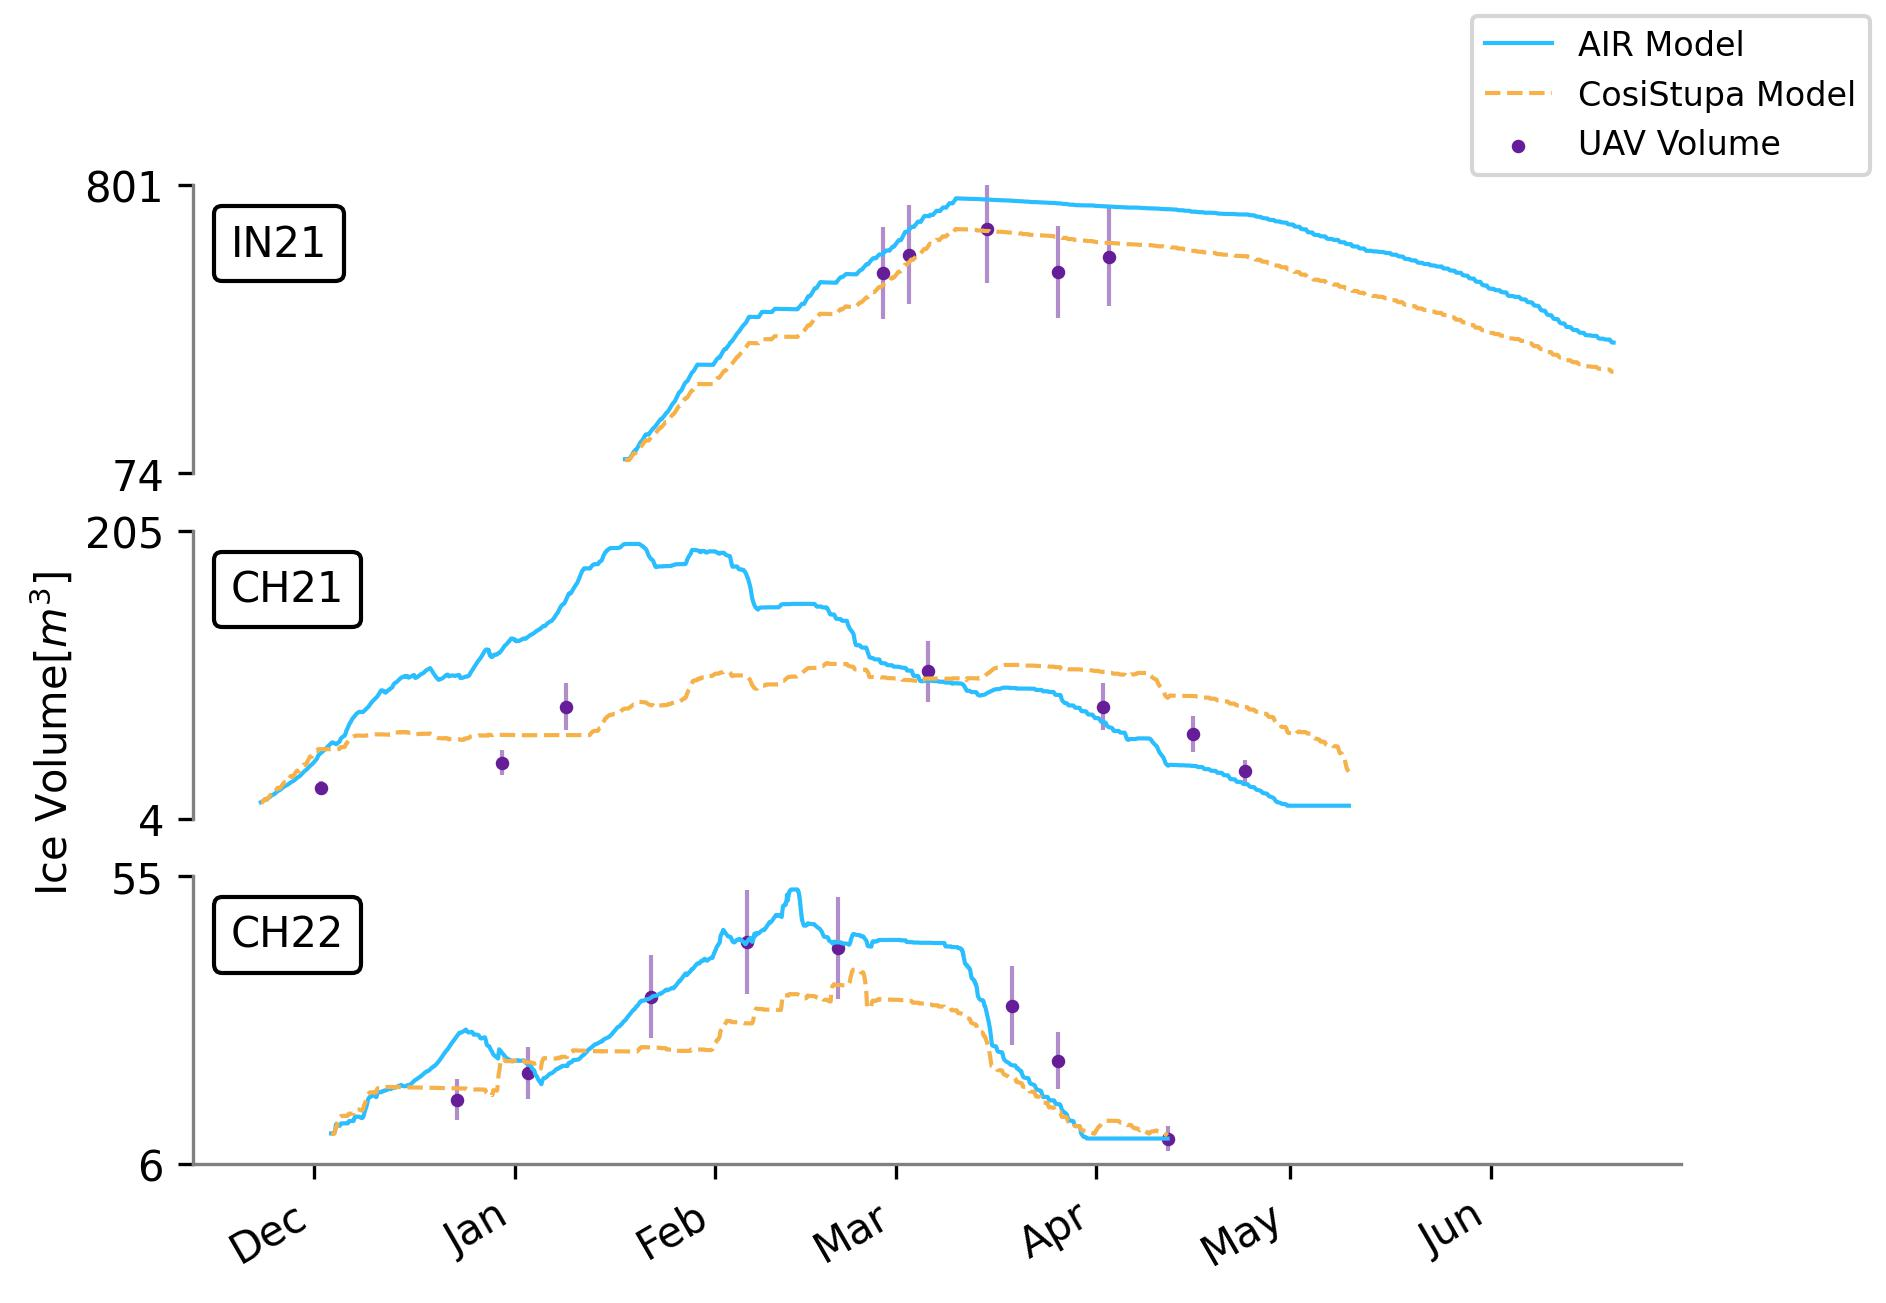
\includegraphics[width=\textwidth]{figs/model_compare.jpg}

	\caption{Comparison of volume estimates generated from the AIR and COSISTUPA models.}

	\label{fig:Cosistupa}
\end{figure}

The COSISTUPA model is considered to be the best one among the three models for the following reasons:

\begin{itemize}

	\item \textbf{Better spatial temperature and density resolution}: The COSISTUPA model provides temperature and density
	      information of subsurface layers of the AIR. In contrast, the AIR model computes only the bulk and the
	      surface temperature. Moreover, COSISTUPA is better able to approximate bulk density since it has records of
	      previous snowfall events in its subsurface layers.

	\item \textbf{Better parametrization of snowfall}: The densification and albedo decay of snowfall are better
	      handled in COSISTUPA due to its awareness of the snowfall content in each of its subsurface layers.

	\item \textbf{Better validation}: COSISTUPA, being derived from COSIPY, is expected to validate better
	      since the core parametrizations are unchanged and have been extensively validated within other studies \citep{arndtAtmosphereDrivenMassBalance2021}.

	\item \textbf{Future support}: COSISTUPA will be extensively supported in the future through the COSIPY
	      community.

\end{itemize}


